\documentclass[12pt]{beamer}

\AtBeginSection[]
{
  \begin{frame}
  \frametitle{Where are we?}
  \tableofcontents[currentsection]
\end{frame}
}

\usetheme{Singapore}

\title{MIFARE Classic Exploits}
\author{Julius Putra Tanu Setiaji}
\date{2 November 2018}

\begin{document}
	\frame{\titlepage}

\begin{frame}
\frametitle{Disclaimer}
The author isn't responsible by the use of the presented content to do illegal activities. Do it at your own risk! 
\end{frame}
	
\section{RFID and NFC}

\begin{frame}
\frametitle{RFID (Radio-frequency identification)}
\begin{itemize}
	\item Uses electromagnetic fields to automatically identify and track tags containing electronically-store information.
	\item Passive tags collect energy from a nearby RFID reader's interrogating radio waves.
	\item Active tags have a local power source and may operate hundreds of meters from the RFID reader.
	\begin{center}
		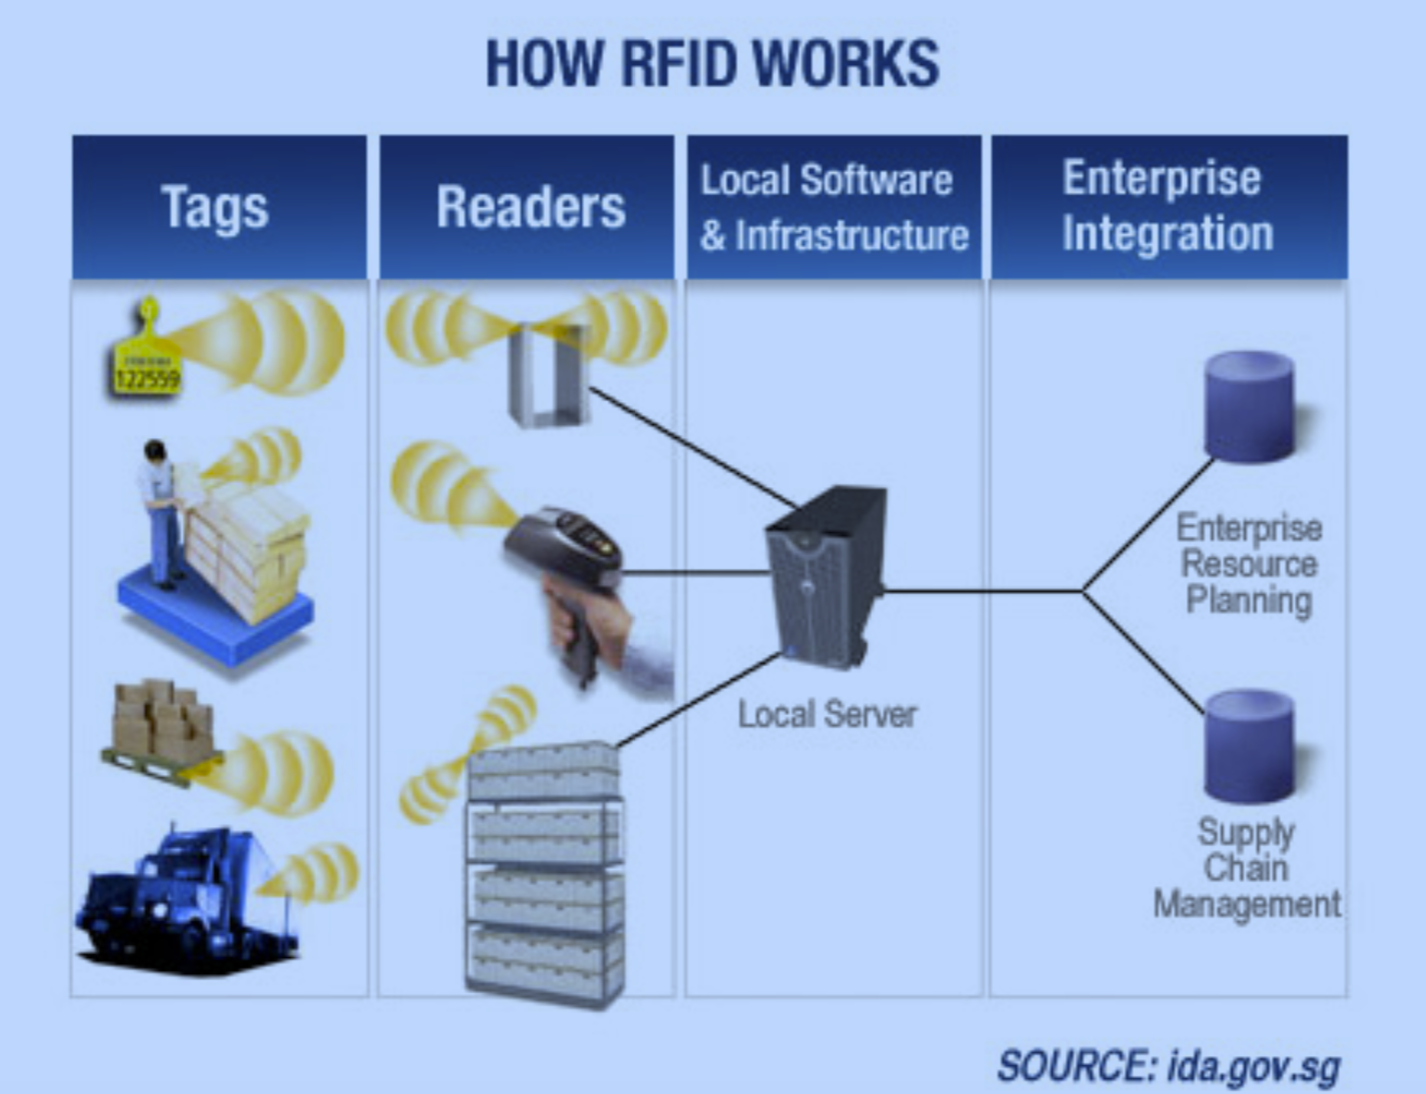
\includegraphics[width=0.5\linewidth]{rfid}
	\end{center}
\end{itemize}
\end{frame}

\begin{frame}
\frametitle{NFC (Near Field Communiation)}
\begin{itemize}
	\item A subset of RFID with much shorter communication ranges.
	\item Unlike most RFID reader-tag pairs, they are able to function as both a reader and a tag:
	\begin{enumerate}
		\item Card Emulation Mode (Android/Apple Pay)
		\item \textbf{Reader/Writer Mode}
		\item Peer to Peer Mode (Android Beam)
	\end{enumerate}
\end{itemize}
\end{frame}

\section{MIFARE Classic}
\begin{frame}
\frametitle{MIFARE}
\begin{itemize}
	\item MIFARE is a group of chips introduced by NXP Semiconductors that is used widely in contactless smart cards.
	\item Introduced in 1995, it is most commonly used in public transportation, access control and ticketing systems.
	\item There are 4 types:
	\begin{enumerate}
		\item \textbf{MIFARE Classic}
		\item MIFARE Plus (AES-128)
		\item MIFARE Ultralight
		\item MIFARE DESFire (DES, 3DES)
	\end{enumerate}
\end{itemize}
\end{frame}

\begin{frame}
\frametitle{MIFARE Classic}
\begin{itemize}
	\item The MIFARE Classic card is generally a memory storage device, where its memory is divided into segments and blocks.
	\item There are 3 types of MIFARE Classic cards:
	\begin{enumerate}
		\item \textbf{MIFARE Classic 1K} (most common)
		\item MIFARE Classic 2K
		\item MIFARE Classic 4K
	\end{enumerate}
	\item Compliant with parts 1-3 (out of 4) of ISO/IEC 14443
	\item Operating at 13.56 MHz with range of up to 10 cm
	\item Proprietary protocol for authentication and ciphering (CRYPTO-1)
	\item 4 bytes UID
\end{itemize}
\end{frame}

\begin{frame}
\frametitle{MIFARE Classic 1K}
\begin{itemize}
	\item 1024 bytes, split into 16 sectors (of 64 bytes each), each divided into 4 blocks (of 16 bytes each).
	\item Each sector is protected by two different keys, each 6-bytes long and 4-bytes Access Condition specifier.
	\item Effectively only 752 bytes are available.
	\begin{center}
		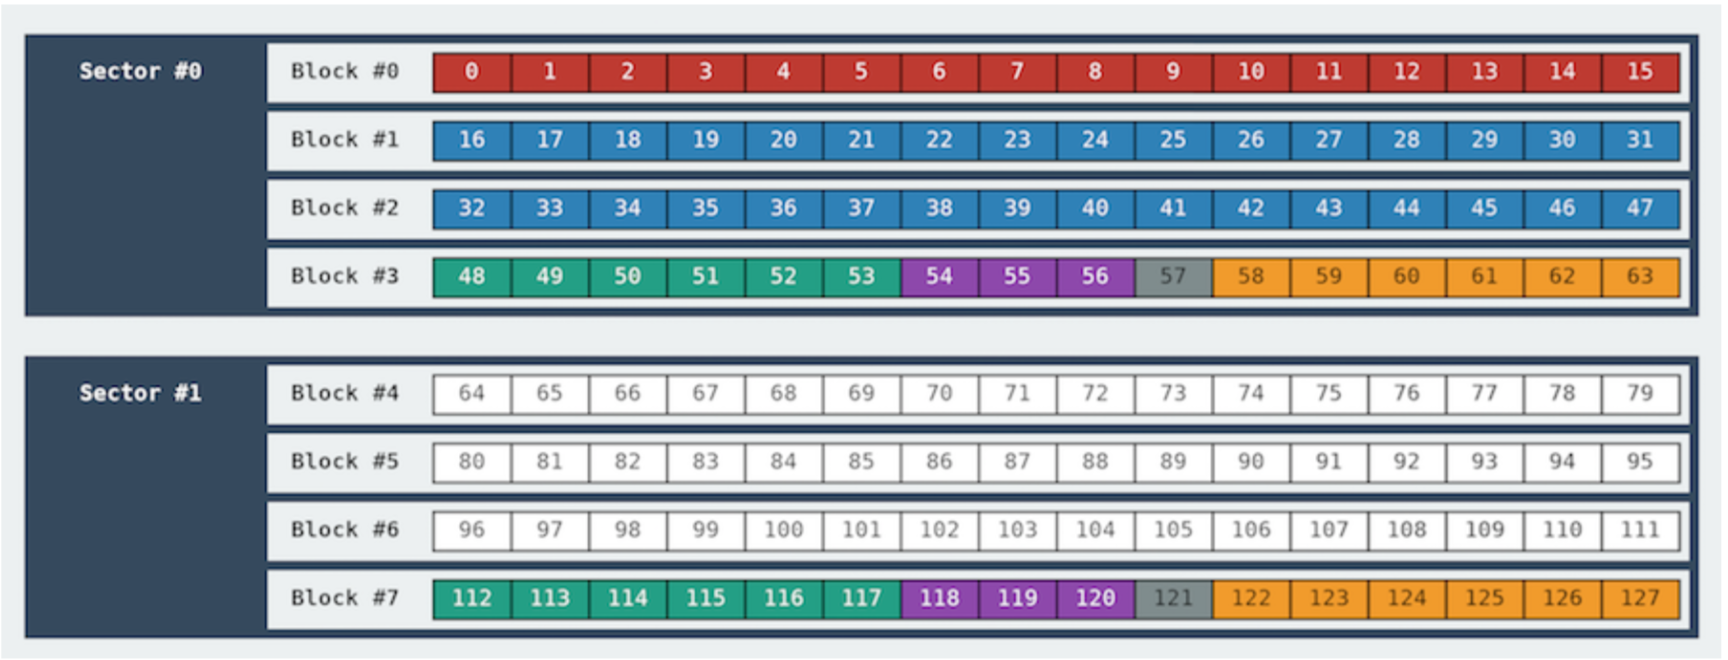
\includegraphics[width=0.85\linewidth]{mfc-sectors} 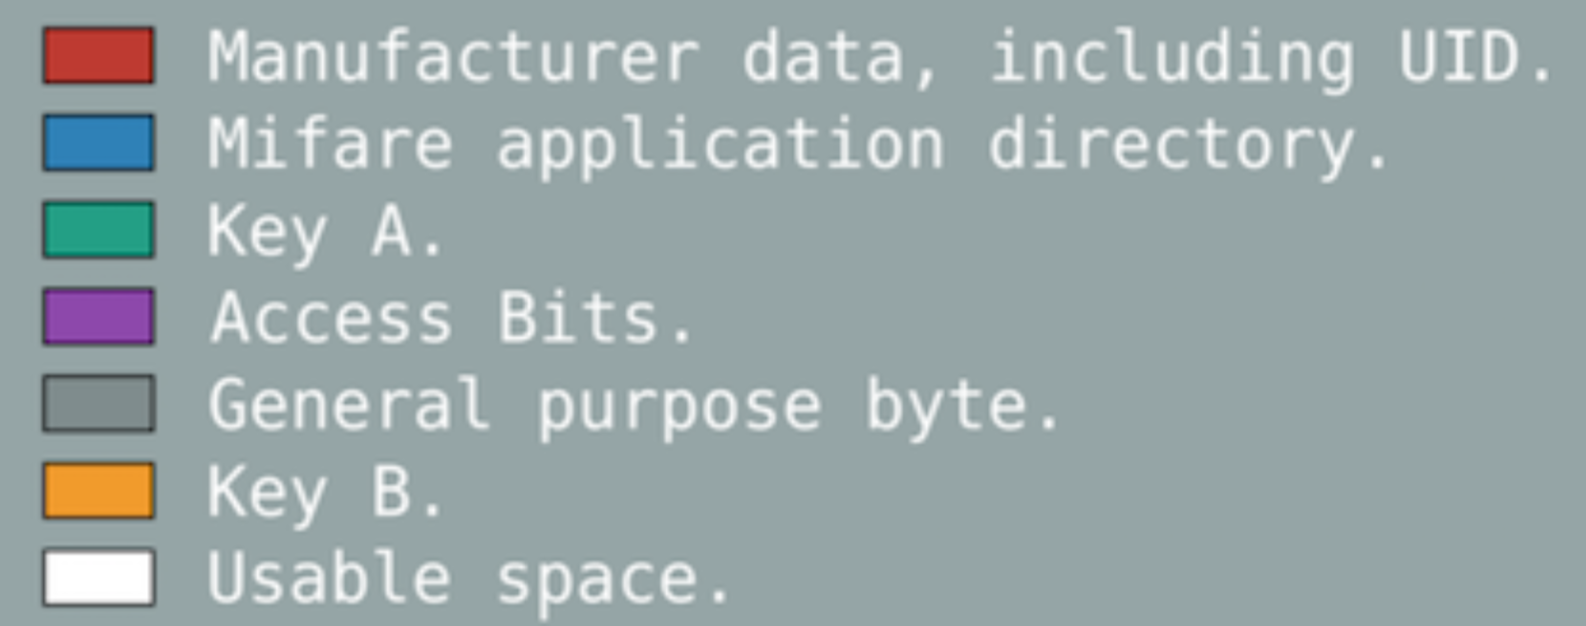
\includegraphics[width=0.35\linewidth]{mfc-sectors-legend}
	\end{center}
\end{itemize}
\end{frame}

\begin{frame}
\frametitle{Manufacturer Block}
\begin{itemize}
	\item First block of sector 0 is known as Manufacturer Block.
	\item First 4 bytes are the UID, next byte is BCC (Bit Count Check -- XOR of the UID bytes).
	\item the remaining eleven bytes are used to store the manufacturer's data.
	\item This further reduces the available space to 752 bytes.
	\item This block is written to and locked in the factory, thus preventing modification.
	\begin{center}
		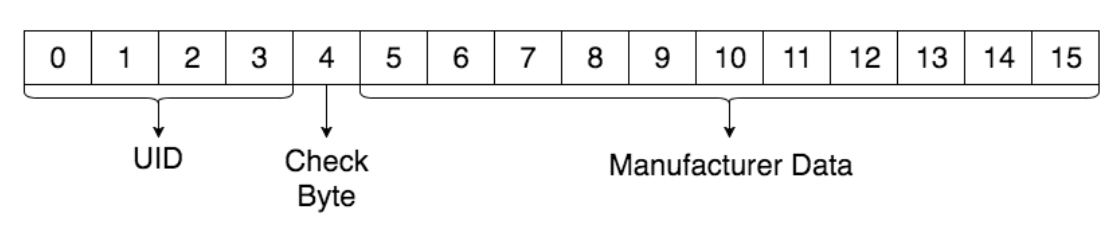
\includegraphics[width=\linewidth]{manufacturer-block}
	\end{center}
\end{itemize}
\end{frame}

\begin{frame}
\frametitle{Sector Trailer}
\begin{itemize}
	\item Block 3 of each sector is called the Sector Trailer.
	\item Used to store 2 secret keys, Key A and Key B of 6 bytes each.
	\item Bytes 6-9 are used to store the access bits meant for accessing the four blocks in each sector.
	\begin{center}
		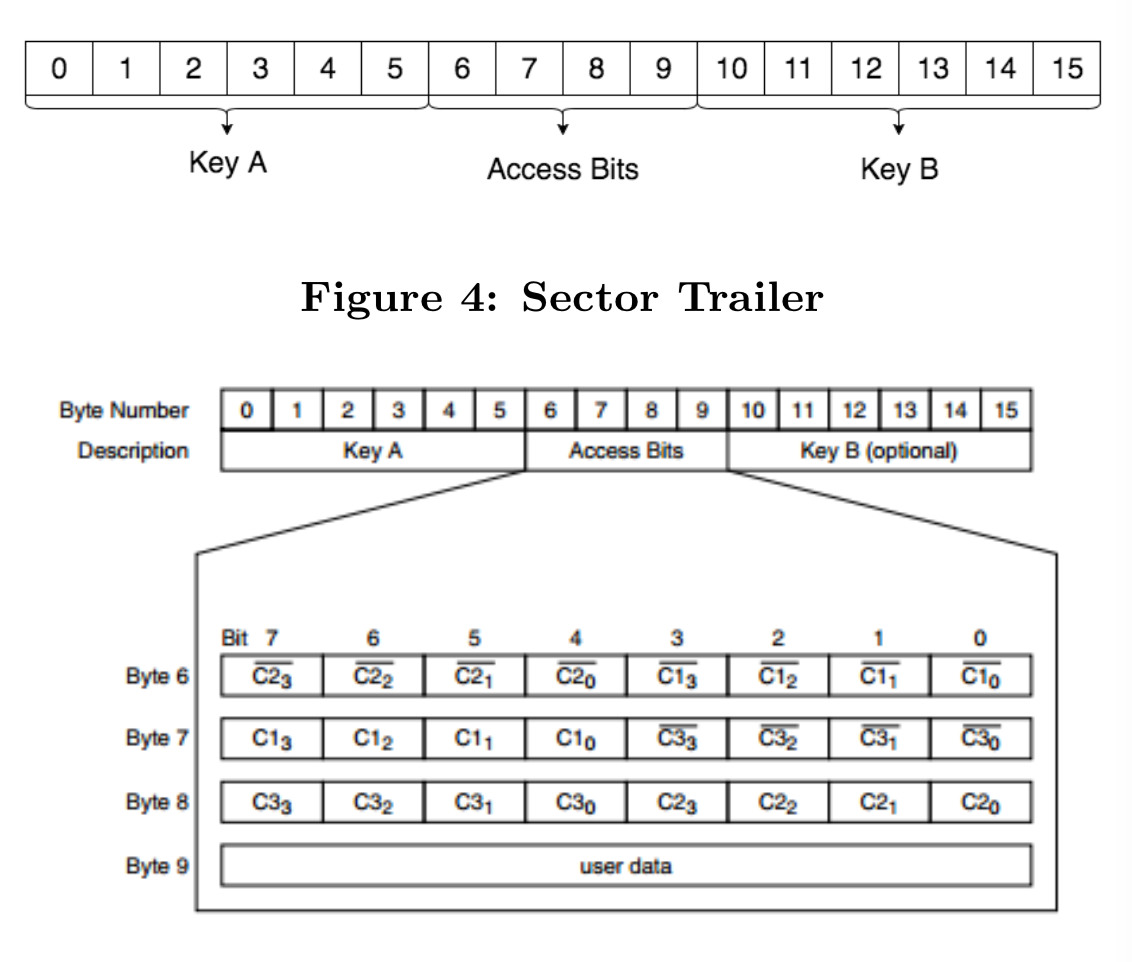
\includegraphics[width=0.45\linewidth]{sector-trailer}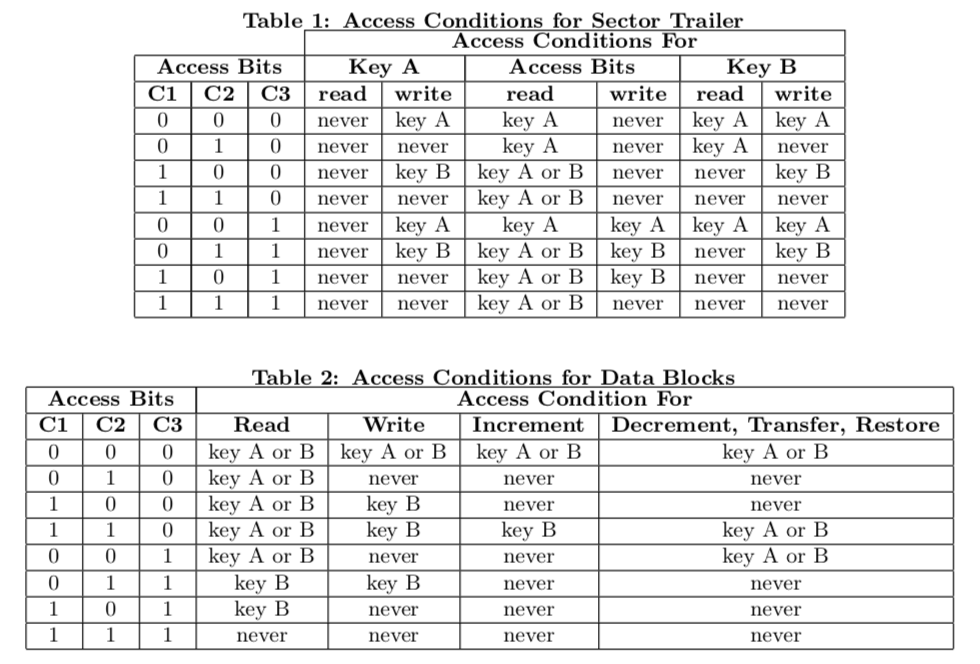
\includegraphics[width=0.55\linewidth]{access-condition}
	\end{center}
\end{itemize}
\end{frame}

\begin{frame}
\frametitle{Short history of CRYPTO-1}
\begin{itemize}
	\item In December 2007, two German researchers (Nohl and Pl{\"o}tz) presented at CCC the partial reverse engineering of Crypto-1 with some weaknesses.
	\item They partially reverse-engineered by slicing the chip and taking pictures using a microscope.
	\item In March 2008, a research group from Radbond University completely reverse-engineered the Crypto-1 cipher by analysing the communication between the tag and the reader.
	\item They intended to publish it, however NXP tried stop the full disclosure of Crypto-1 cipher by judicial process.
	\item However, in July 2008 the court decides allow the publication of the paper and reject the prohibition based on freedom of speech principles.
\end{itemize}
\end{frame}

\begin{frame}
\frametitle{CRYPTO-1 (1/3)}
\begin{center}
  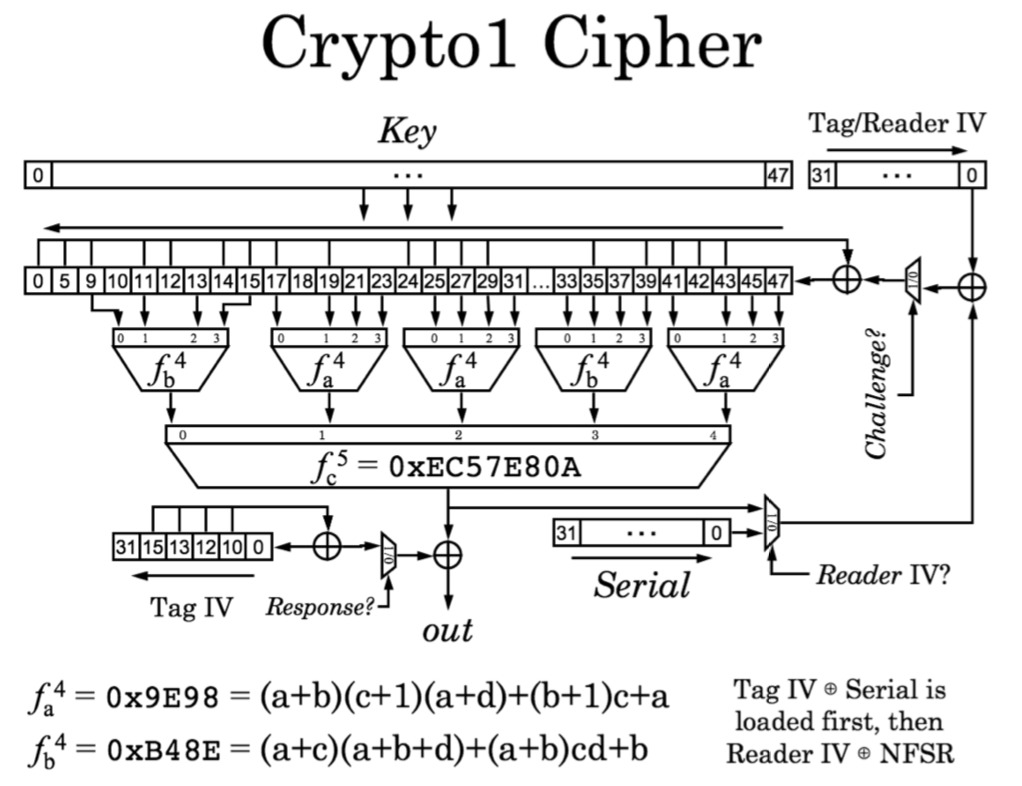
\includegraphics[width=0.5\linewidth]{crypto-1}
  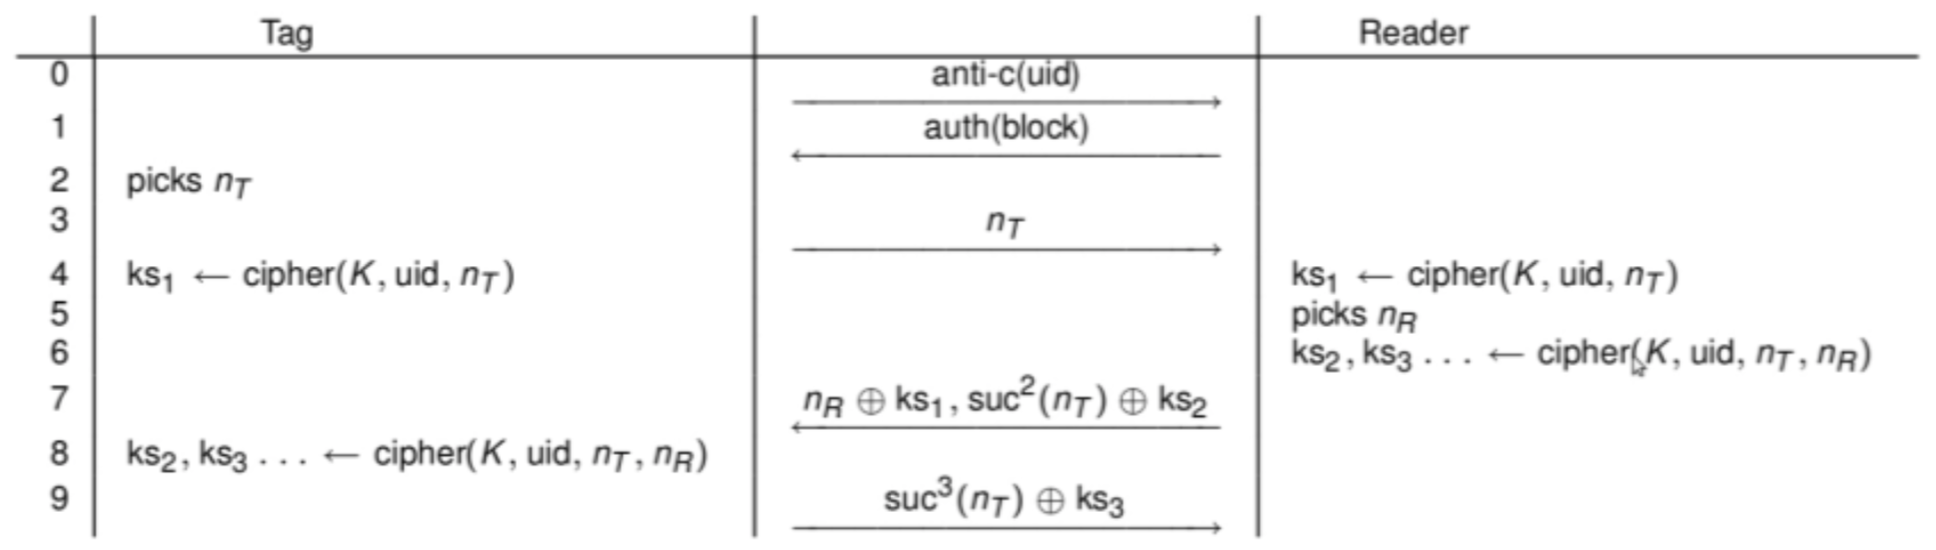
\includegraphics[width=0.7\linewidth]{card-comm}
\end{center}
\end{frame}

\begin{frame}
\frametitle{CRYPTO-1 (2/3)}
\begin{itemize}
	\item A stream cipher that uses a 48-bit secret key.
	\item The card sends a challenge nonce $n_T$, after which the reader sends the encrypted reader nonce $n_R\oplus ks_1$ and challenge response $suc^2(n_T)\oplus ks_2$.
	\item The 3-way authentication is completed when the card sends the encrypted challenge response $suc^3(n_T)\oplus ks_3$.
	\item The 32 bit nonces are generated by a 16 bit linear feedback shift register (LSFR).
	\item In this case, $suc(x)$ refers to the next 32 bits generated by the LSFR after $x$.
	\item $ks_1, ks_2, ks_3$ are key stream generated by cipher (32 bits each.)
\end{itemize}
\end{frame}

\begin{frame}
\frametitle{CRYPTO-1 (3/3)}
\begin{itemize}
	\item At the heart is a 48 bit feedback shift register which is initialized with with the secret key $K$, the uid and the $n_T$, and later $n_R$ is fed in.
	\item 20 bits of the feedback shift register are used as input to a filter function to generate the keystream.
	\item The researchers were able to invert the filter function so as to effectively generate all the possible internal states of the feedback shift register given a partial keystream.
\end{itemize}
\end{frame}

\section{Protocol Weaknesses}
\begin{frame}
\frametitle{Replay Attack and Active Sniffing}
\begin{itemize}
	\item After the 2008 publication of the full CRYPTO-1 cipher, any attacker is able to emulate any Mifare card by just sniffing the communication between the card and reader and replaying it (including the UID value).
	\item Also, the attacker will be able to recover all keys from sectors involved in this communication.
	\item However, this attack needs to sniff the communication between the card and a valid reader.
	\item The hardware required are also rather expensive and not easily accessible.
\end{itemize}
\end{frame}

\begin{frame}
\frametitle{Parity Bits (1/2)}
\begin{itemize}
  \item MIFARE Classic sends a parity bit for each byte it transmits.
  \item However, contrary to the ISO 14443-A standard, the data link layer and communication layer are mixed.
  \item Instead of computing parity bits over the ciphertext, they are computed over the plaintext.
  \item Moreover, the parity bits are sent encrypted with the same keystream bit used to encrypt the next bit of plaintext.
\end{itemize}
\end{frame}

\begin{frame}
\frametitle{Parity Bits (2/2)}
\begin{center}
  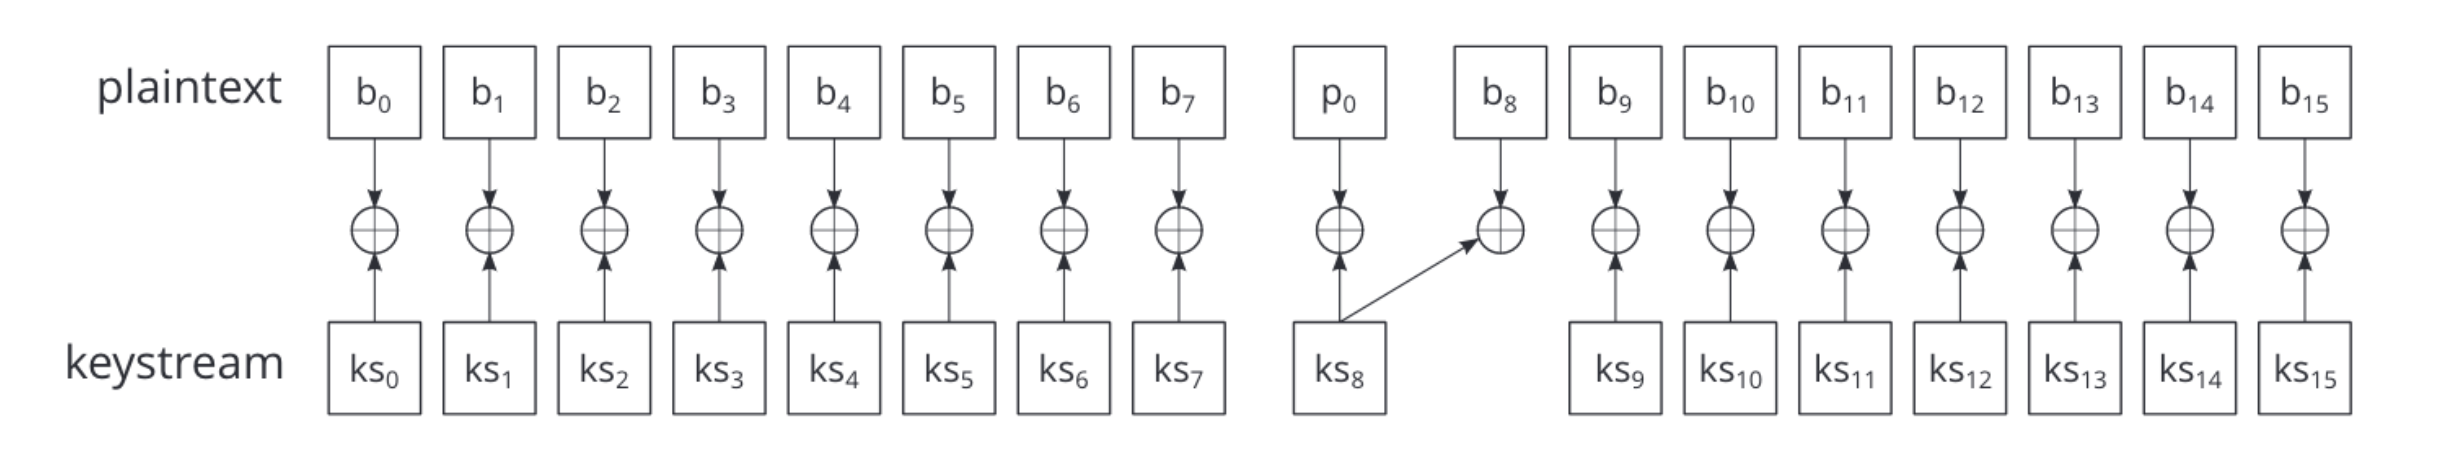
\includegraphics[width=\linewidth]{darkside}
\end{center}
\begin{itemize}
  \item Observe the encrypted parity bit $p_0$ of $n_{T_{[0, 7]}}$ and encrypted bit $b_8$ from $n_{T_8}$. Since both are encrypted using the same keystream bit $ks_8$, we can deduce whether the plaintext parity $p_0$ equals $n_{T_8}$
  \item This requires no knowledge about CRYPTO1 other than it is a stream cipher which encrypts bitwise.
\end{itemize}
\end{frame}

\begin{frame}
\frametitle{Other Weaknesses}
\begin{itemize}
  \item The keys are only 48-bits long. Can be brute-forced with FPGA, approximately 10 hours to recover one key.
  \item The LFSR used by the RNG is predictable (constant initial condition, and generated by a 16-bit LFSR -- only 16 bits of entropy)
  \item Each random number only depends of the quantity of clock cycles between: the time when the reader was turned up and the time when the random number is requested.
  \item Since an attacker controls the time of protocol, one is able to control the generated random numbers and that way recover the keys from communication.
\end{itemize}
\end{frame}

\section{Darkside Attack}
\begin{frame}
\frametitle{Darkside Attack}
\begin{itemize}
  \item Introduced in 2009 by Nicolas Courtois and implemented by Andrei Costin with the \texttt{MFCUK}.
  \item During the 3-step authentication, when the reader sends $n_R\oplus ks_1$ and $suc^2(n_T)\oplus ks_2$, the tag checks the 8 parity bits before checking the correctness of $suc^2(n_T)\oplus ks_2$.
  \item If the parity bits for these 8 bytes are correct but $suc^2(n_T)\oplus ks_2$ is wrong, the card will respond with a 4-bit encrypted error code (NACK -- \texttt{0x5}) indicating a transmission error, \texttt{0x5} $\oplus k$ where $k$ is the first 4 bits of $ks_3$.
  \item If the parity bits are wrong, the card does not respond.
  \item This allows the attacker to correctly guess 4 bits of the keystream after an average of $2^8$ tries (for the 8 parity bits).
\end{itemize}
\end{frame}



\section{Nested Attack}
\begin{frame}
\frametitle{Nested Attack (1/2)}
\begin{itemize}
	\item Recover all keys after at least one key has been found, taking advantage of the weakness in the PRNG used to generate the nonce.
  \item The weak PRNG allows an adversary to predict the nonce, and then using it to recover 32 bits of keystream.
	\item Introduced in 2009 by Nijmegan Oakland and Implemented by Nethemba with the \texttt{mfoc} tool.
\end{itemize}
\end{frame}

\begin{frame}
\frametitle{Nested Attack (2/2)}
\begin{itemize}
  \item First, authenticate to a sector with a known key.
  \item When attempting to authenticate to another sector, the card will send encrypted challenge $n_T\oplus k'$ where $n_T$ is the nonce and $k'$ is the keystream generated by the key of the new sector (encrypted using the key of the new sector).
  \item PRNG has only a 16-bit state, and parity bits leak 3 bits of information, allowing an adversary to guess the nonce and recover 32 bits of keystream.
  \item From the invertibility of the filter function, each correctly guessed nonce will result in a set of possible candidate keys (approximately $2^16$ candidate keys). An intersection of these sets will quickly find the required secret key.
\end{itemize}
\end{frame}

\begin{frame}
\frametitle{Less cheem explanation}
\begin{itemize}
	\item Authenticate to a block with known key and read $n_T$ (determined by LFSR)
	\item Authenticate to the same block again with the default key and read $n_T'$ (determined by LFSR)
	\item Compute the number of LFSR shifts ("timing distance")
	\item Guess the next $n_T$ value, calculate $ks_1, ks_2, ks_3$ and try authenticating to a different block.
\end{itemize}
\end{frame}

\section{Hard-nested Attack}
\begin{frame}
\frametitle{Hardened MIFARE Classic Cards}
\begin{itemize}
	\item In light of this, many manufactures and system integrators started to deploy "fixed" mifare Classic cards which are resilient
	to such vulnerabilities, especially the weak PRNG.
	\item However, these countermeasures
	are inadequate for a cryptographically insecure cipher such as CRYPTO-1.
	\item Instead of taking advantage of the MIFARE protocol and its implementations (non-cryptographically related implementation
	flaws), researchers look into breaking the CRYPTO-1 cipher itself.
\end{itemize}
\end{frame}

\begin{frame}
\frametitle{Collecting nonces stage (1/2)}
\begin{itemize}
	\item The information obtained allows an attacker to drop the computational complexity from $2^{48}$ to approximately $2^{30}$
	\item Retrieve encrypted nonces $n_T$ using the nested authentication, i.e. by authenticating for a sector with a known key, followed by an authentication request for the request for the target sector.
	\item Given the set of encrypted nonces obtained so far, determine sum property of the cipher's initial state $S_e$ and of the cipher's state after byte $b$ is fed, $S_b$ for all 256 possible first input bytes $b$.
	\item Depending on the probability that we guessed $S_b$ correctly (using a probability threshold value), incorporate byte $b$ in the differential analysis, and incorporate all first nonce bytes for which the filter flip property holds.
\end{itemize}
\end{frame}

\begin{frame}
\frametitle{Collecting nonces stage (2/2)}
\begin{itemize}
	\item Given the information determined from the set of encrypted nonces, we determine the size of the leftover search space.
	\item The leftover search space shrinks as the number of harvested encrypted nonces increases since more nonces allows us to more accurately guess sum properties and observe filter flip properties.
	\item When the search space is sufficiently small, we construct a candidate list for $a_{[9,55]}$, extended to $a_{[8,55]}$, then performing an LFSR-rollback to transform them into candidates for $a_{[0,47]}$, i.e. the secret key.
\end{itemize}
\end{frame}

\begin{frame}
\frametitle{Brute-force Stage}
\begin{itemize}
	\item This candidates list can then be used for offline brute force attack (which can be parallelised!)
	\item Parity bits are computed over plaintext byte XOR-ed with the next keystream bit. This property can be exploted to verify whether a candidate key is the correct key.
	\item Given an encrypted nonce obtained through
	a nested authentication attempt, the attacker can attempt to "decrypt" the nonce using the candidate key.
	\item In case the candidate is the correct key, the parity bits will be correct. However, in case a wrong key was used, a parity bit will be
	correct with probability $\frac{1}{2}$
	\item If the key is not found, revert to Stage 2 optionally with an increased probability threshold. However, gathering of more nonces increases the certainty and reduces the number of candidate keys.
\end{itemize}
\end{frame}

\begin{frame}
\frametitle{Further Reading}
\begin{itemize}
	\item The offline brute-forcing part can be improved by using bit-slicing, achieving 8-10 times speedup. (\url{https://github.com/aczid/crypto1_bs})
	\item Details about this attack is available on this paper: \url{http://www.cs.ru.nl/~rverdult/Ciphertext-only_Cryptanalysis_on_Hardened_Mifare_Classic_Cards-CCS_2015.pdf}
\end{itemize}
\end{frame}

\section{Conclusion}
\begin{frame}
\frametitle{Closing Statements}
\begin{itemize}
	\item MIFARE Classic practically offers no security all, just like WEP for the Wi-Fi standard.
	\item Moreover, in reality, there are other ways to defeat MIFARE Classic security system.
	\item For example, some MIFARE Classic cards from China allows first block of sector 0 (Manufacturer Block) to be rewritten. This defeats some systems that bases identification on UID.
\end{itemize}
\end{frame}

\begin{frame}
\frametitle{Live Demonstration}
\begin{center}
  Thank you very much.
\end{center}
\end{frame}
\end{document}